
\documentclass{beamer}		% This tells LaTeX the document will be a "beamer" presentation

\mode<presentation>
{
  \usetheme{Madrid}      % or try Darmstadt, Madrid, Warsaw, ...
  \usecolortheme{default} % or try albatross, beaver, crane, ...
  \usefonttheme{serif}  % or try serif, structurebold, ...
  \setbeamertemplate{navigation symbols}{}
  \setbeamertemplate{caption}[numbered]
} 

\usepackage{amsmath}
\usepackage{amssymb}
\usepackage{amsfonts}
\usepackage{bm}
\usepackage{graphicx}

\usepackage[backend=bibtex,sorting=none]{biblatex}
\addbibresource{references.bib}
\setbeamerfont{footnote}{size=\tiny}
\setbeamertemplate{bibliography item}[text]
\newcommand{\dd}{\mathrm{d}}
\newcommand{\R}{\mathbb{R}}
\newcommand{\E}{\mathbb{E}}

\title[RetCL]{RetCL: A Selection-based Approach for Retrosynthesis via Contrastive Learning}	% Insert your title.  Depending on the theme you choose above, a "short title" might be useful, as it will appear on the footer of each slide.

\author[Shen Yuan]{Hankook Lee \quad Sungsoo Ahn \quad Seung-Woo Seo \quad You Young Song \quad Eunho Yang \quad Sung-Ju Hwang \quad Jinwoo Shin} % Insert your name

% \institute[UoE]{University of Edinburgh} % Self-explanatory



\begin{document} 	% Let's begin

% Presentations come in slide frames.  You have to tell LaTeX when to start a frame, and when to end the frame.  The most common error beginners make with beamer is forgetting the \end{frame} command.	

\newcommand{\light}[1]{\textcolor{gray}{#1}}

\begin{frame}	

\titlepage	% Prints a title page populated with the information given in the preamble
	
\end{frame}	



\begin{frame}[noframenumbering]
\begin{itemize}
    \begin{LARGE}
    \item Introduction
    \item \light{Search procedure}
    \item \light{Training scheme with contrastive learning}
    \item \light{Experiments}
    \end{LARGE}
\end{itemize}
\end{frame}



\begin{frame}{Notation}

\begin{itemize}
    \item $P,R$: product and reactant molecules.
    \item $\mathcal{C}$: the candidate set.
    \item $\mathcal{R}$: the reactant set.
    \item $\prod$: the space of permutations.
\end{itemize}

\end{frame}



\begin{frame}{Introduction}

The RetCL framework:

\begin{itemize}
    \item selection-based
    \item template-free
\end{itemize}

\end{frame}



\begin{frame}{The Search Procedure of RetCL}

\begin{figure}[t]
\centerline{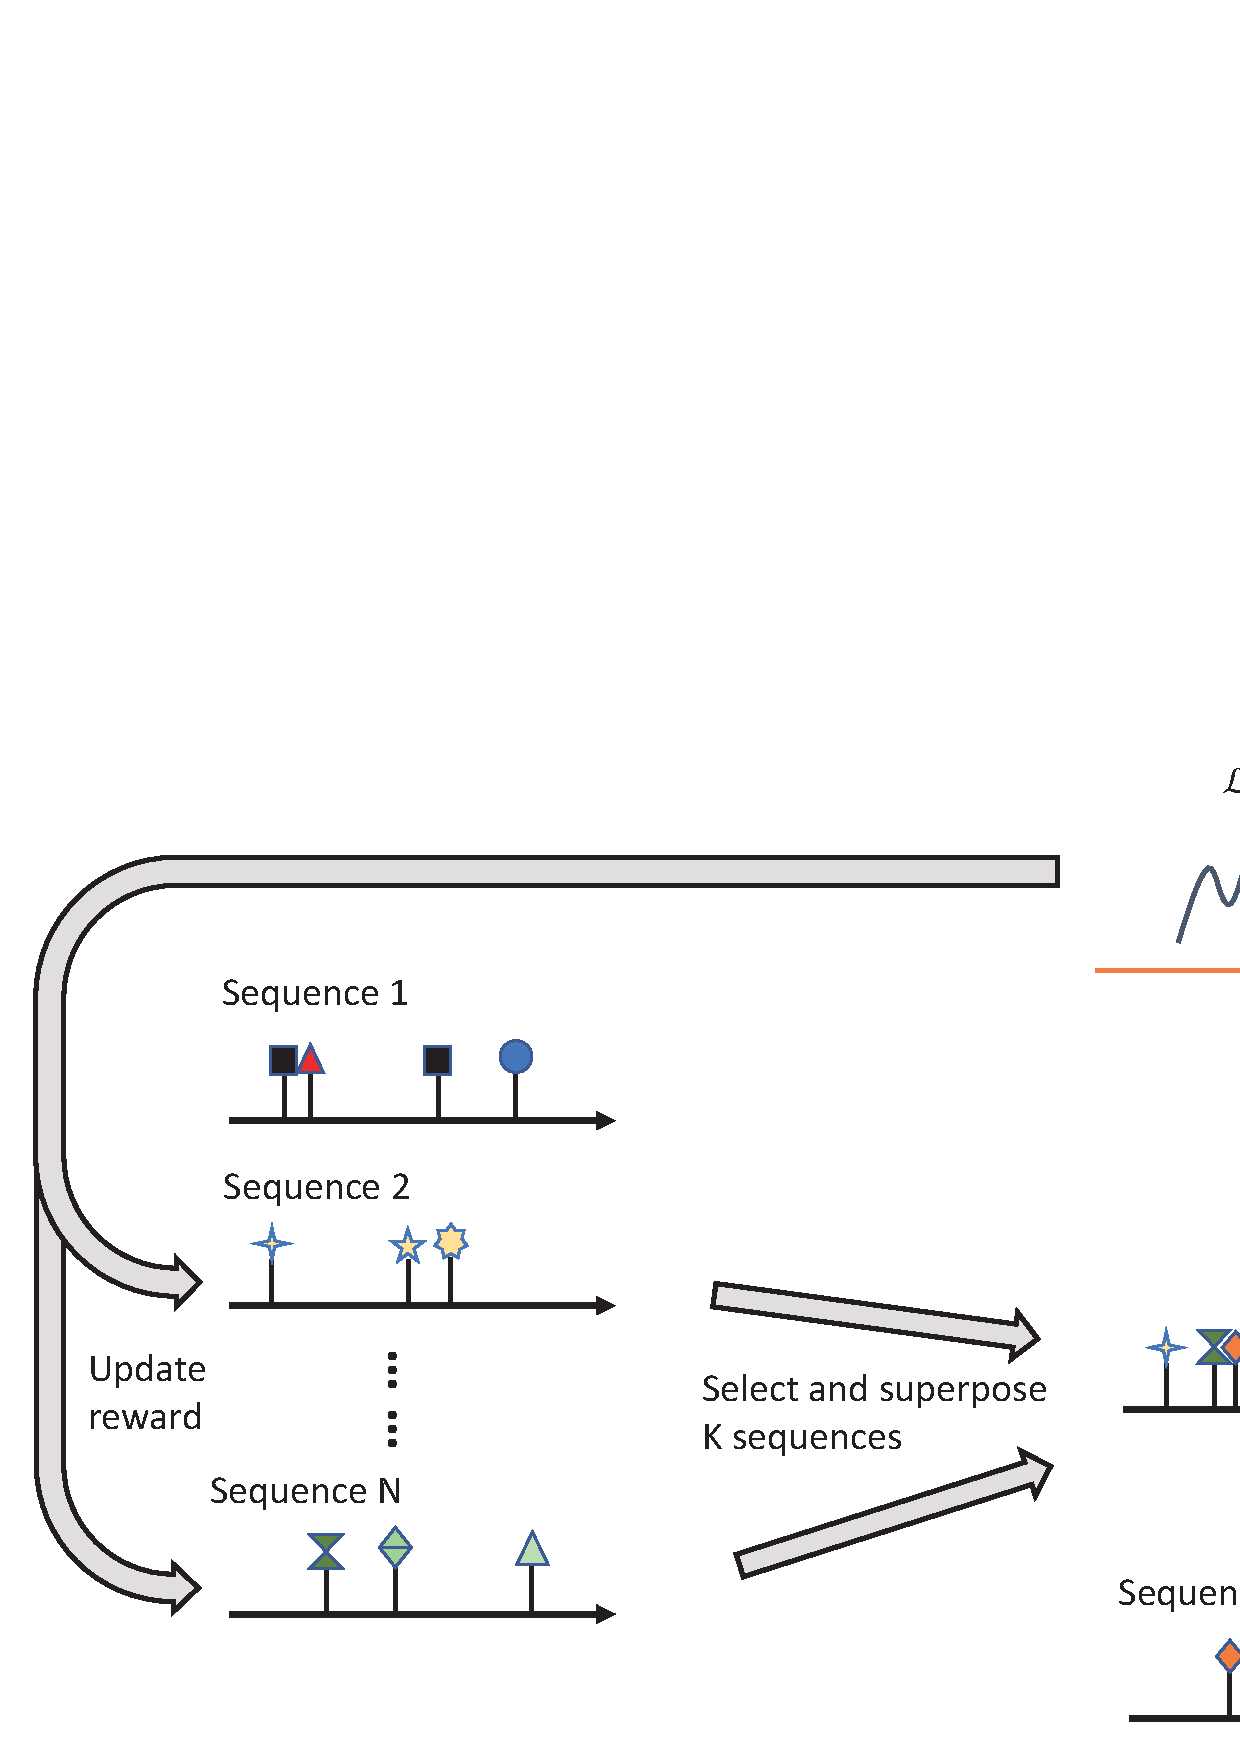
\includegraphics[width=1.0\linewidth]{figure1.jpg}}
\vspace{-10pt}
\caption{Illustration of the search procedure in RetCL.}
\label{fig1}
\end{figure}
    
\end{frame}



\begin{frame}[noframenumbering]
\begin{itemize}
    \begin{LARGE}
    \item \light{Introduction}
    \item Search Procedure
    \item \light{Training Scheme with Contrastive Learning}
    \item \light{Experiments}
    \end{LARGE}
\end{itemize}
\end{frame}



\begin{frame}{Search Procedure}

\begin{itemize}
    \item \textbf{Object}: To find a reactant-set $\mathcal{R}=\{R_1,\ldots,R_n\}$
    \item \textbf{Input}: The product $P$ and the candidate set $\mathcal{C}$
    \item First, select each reactant $R_i$ sequentially from the candidate set $\mathcal{C}$ based on the backward selection score $\psi(R|P, \mathcal{R}_{\text{given}})$.
    \item Then, repeat the first step to get many reactant-sets.
    \item Finally, rank the chosen reactant-sets $\mathcal{R}_1, \ldots, \mathcal{R}_T$ based on the backward selection score $\psi(R|P, \mathcal{R}_{\text{given}})$ and the forward score $\phi(P|\mathcal{R})$.
\end{itemize}

\end{frame}



\begin{frame}{Score Design}

\begin{eqnarray*}
\begin{aligned}
\psi(R|P, \mathcal{R}_{\text{given}}) =\text{CosSim} \left( f_{\theta}(P)-\sum_{\mathcal{S}\in\mathcal{R}_{\text{given}}} g_{\theta}(S), \  h_{\theta}(R) \right)
\end{aligned}    
\end{eqnarray*}

\begin{eqnarray*}
\begin{aligned}
\phi(P|\mathcal{R}) = \text{CosSim} \left( \sum_{R\in\mathcal{R}} g_{\theta}(R) , \ h_{\theta}(P) \right)
\end{aligned}    
\end{eqnarray*}

where $\text{CosSim}$ is the cosine similarity and $f_\theta, g_\theta, h_\theta$ are embedding functions from a molecule to a fixed-sized vector with parameters $\theta$.

\end{frame}



\begin{frame}{Score Design}

The overall score on a chemical reaction $\mathcal{R} \to P$ is defined as

\begin{eqnarray*}
\begin{aligned}
\text{score}(P, \mathcal{R})=\frac{1}{n+2} \left( \max_{\pi \in \prod} \sum_{i=1}^{n+1} \psi(R_{\pi(i)}|P, \{R_{\pi(1)}, \ldots, R_{\pi(i-1)}\}) + \phi(P|\mathcal{R}) \right)
\end{aligned}    
\end{eqnarray*}

where $R_{n+1}=R_{\text{halt}}$ and $\prod$ is the space of permutations defined on the integers $1, \ldots, n+1$ satisfying $\pi(n+1)=n+1$.

\end{frame}



\begin{frame}[noframenumbering]
\begin{itemize}
    \begin{LARGE}
    \item \light{Introduction}
    \item \light{Search Procedure}
    \item Training Scheme with Contrastive Learning
    \item \light{Experiments}
    \end{LARGE}
\end{itemize}
\end{frame}



\begin{frame}{Two Classification Tasks}

\begin{eqnarray*}
\begin{aligned}
p(R|P, \mathcal{R}_{\text{given}}, \mathcal{C}) = \frac{\text{exp}(\psi(R|P,\mathcal{R}_{\text{given}})/\tau)}{\sum_{R' \in \mathcal{C}\setminus\{P\}} \text{exp}(\psi(R'|P, \mathcal{R}_{\text{given}})/\tau)}
\end{aligned}    
\end{eqnarray*}

\begin{eqnarray*}
\begin{aligned}
q(P|\mathcal{R}, \mathcal{C}) = \frac{\text{exp}(\phi(P|\mathcal{R})/\tau)}{\sum_{P' \in \mathcal{C}\setminus\mathcal{R}} \text{exp}(\phi(P'|\mathcal{R})/\tau)}
\end{aligned}    
\end{eqnarray*}

where $\tau$ is a hyperparameter for temperature scaling and $\mathcal{C}$ is the given candidate set of molecules.

\end{frame}



\begin{frame}{Loss Function}

The Losses defined on a reaction of the product $P$ and the reactant-set $\mathcal{R}=\{R_1,\ldots,R_n\}$:

\begin{eqnarray*}
\begin{aligned}
\mathcal{L}_{\text{backward}}(P, \mathcal{R}|\theta, \mathcal{C}) = -\max_{\pi \in \prod} \sum_{i=1}^{n+1} \text{log} \ p(R_{\pi(i)}|P, \{R_{\pi(1)}, \ldots, R_{\pi(i-1)}\}, \mathcal{C})
\end{aligned}    
\end{eqnarray*}

\begin{eqnarray*}
\begin{aligned}
\mathcal{L}_{\text{forward}}(P, \mathcal{R}|\theta, \mathcal{C}) = -\text{log} \  q(P|\mathcal{R}, \mathcal{C})
\end{aligned}    
\end{eqnarray*}

where $R_{n+1}=R_{\text{halt}}$ and $\prod$ is the space of permutations defined on the integers $1, \ldots, n+1$ satisfying $\pi(n+1)=n+1$.

\end{frame}



\begin{frame}{Candidate Set}

Because the denominators of $p(\cdot)$ and $q(\cdot)$ require summation over the large set of candidate set $\mathcal{C}$. 

For each mini-batch of reactions $\mathcal{B}$ sampled from the training dataset:

\begin{eqnarray*}
\begin{aligned}
\mathcal{C}_{\mathcal{B}} = \{M| \exists (\mathcal{R}, P) \in \mathcal{B} \ \text{such that} \ M=P \ \text{or} \ M \in \mathcal{R}\}
\end{aligned}    
\end{eqnarray*}

\begin{eqnarray*}
\begin{aligned}
\mathcal{L}(\mathcal{B}|\theta) = \frac{1}{|\mathcal{B}|} \sum_{(\mathcal{R}, P) \in \mathcal{B}} \left(\mathcal{L}_{\text{backward}}(P, \mathcal{R}|\theta, \mathcal{C}_{\mathcal{B}}) + \mathcal{L}_{\text{forward}}(P, \mathcal{R}|\theta, \mathcal{C}_{\mathcal{B}})  \right)
\end{aligned}    
\end{eqnarray*}



\end{frame}


\begin{frame}{Hard Negative Mining}

\begin{eqnarray*}
\begin{aligned}
\tilde{\mathcal{C_B}} = \mathcal{C_B} \cup \bigcup_{M\in \mathcal{C_B}} \{\text{Top-K nearest neighbors of M from } \mathcal{C}\}
\end{aligned}    
\end{eqnarray*}

where $K$ is a hyperparameter controlling hardness of the contrastive task. The nearest neighbors are defined with respect to the cosine similarity on $\{h_\theta(M)\}_{M\in\mathcal{C}}$.

\end{frame}



\begin{frame}[noframenumbering]
\begin{itemize}
    \begin{LARGE}
    \item \light{Introduction}
    \item \light{Search Procedure}
    \item \light{Training Scheme with Contrastive Learning}
    \item Experiments
    \end{LARGE}
\end{itemize}
\end{frame}



\begin{frame}{Datasets}

\begin{itemize}
    \item Datasets: USPTO-50k.
    \item The candidate set: choose the candidate set of commercially available molecules $\mathcal{C}$ as the all reactants in the entire USPTO database
    \item Evaluation metric: top-k exact match accuracy.
\end{itemize}
    
\end{frame}



\begin{frame}{The top-k exact match accuracy}

\begin{figure}[t]
\centerline{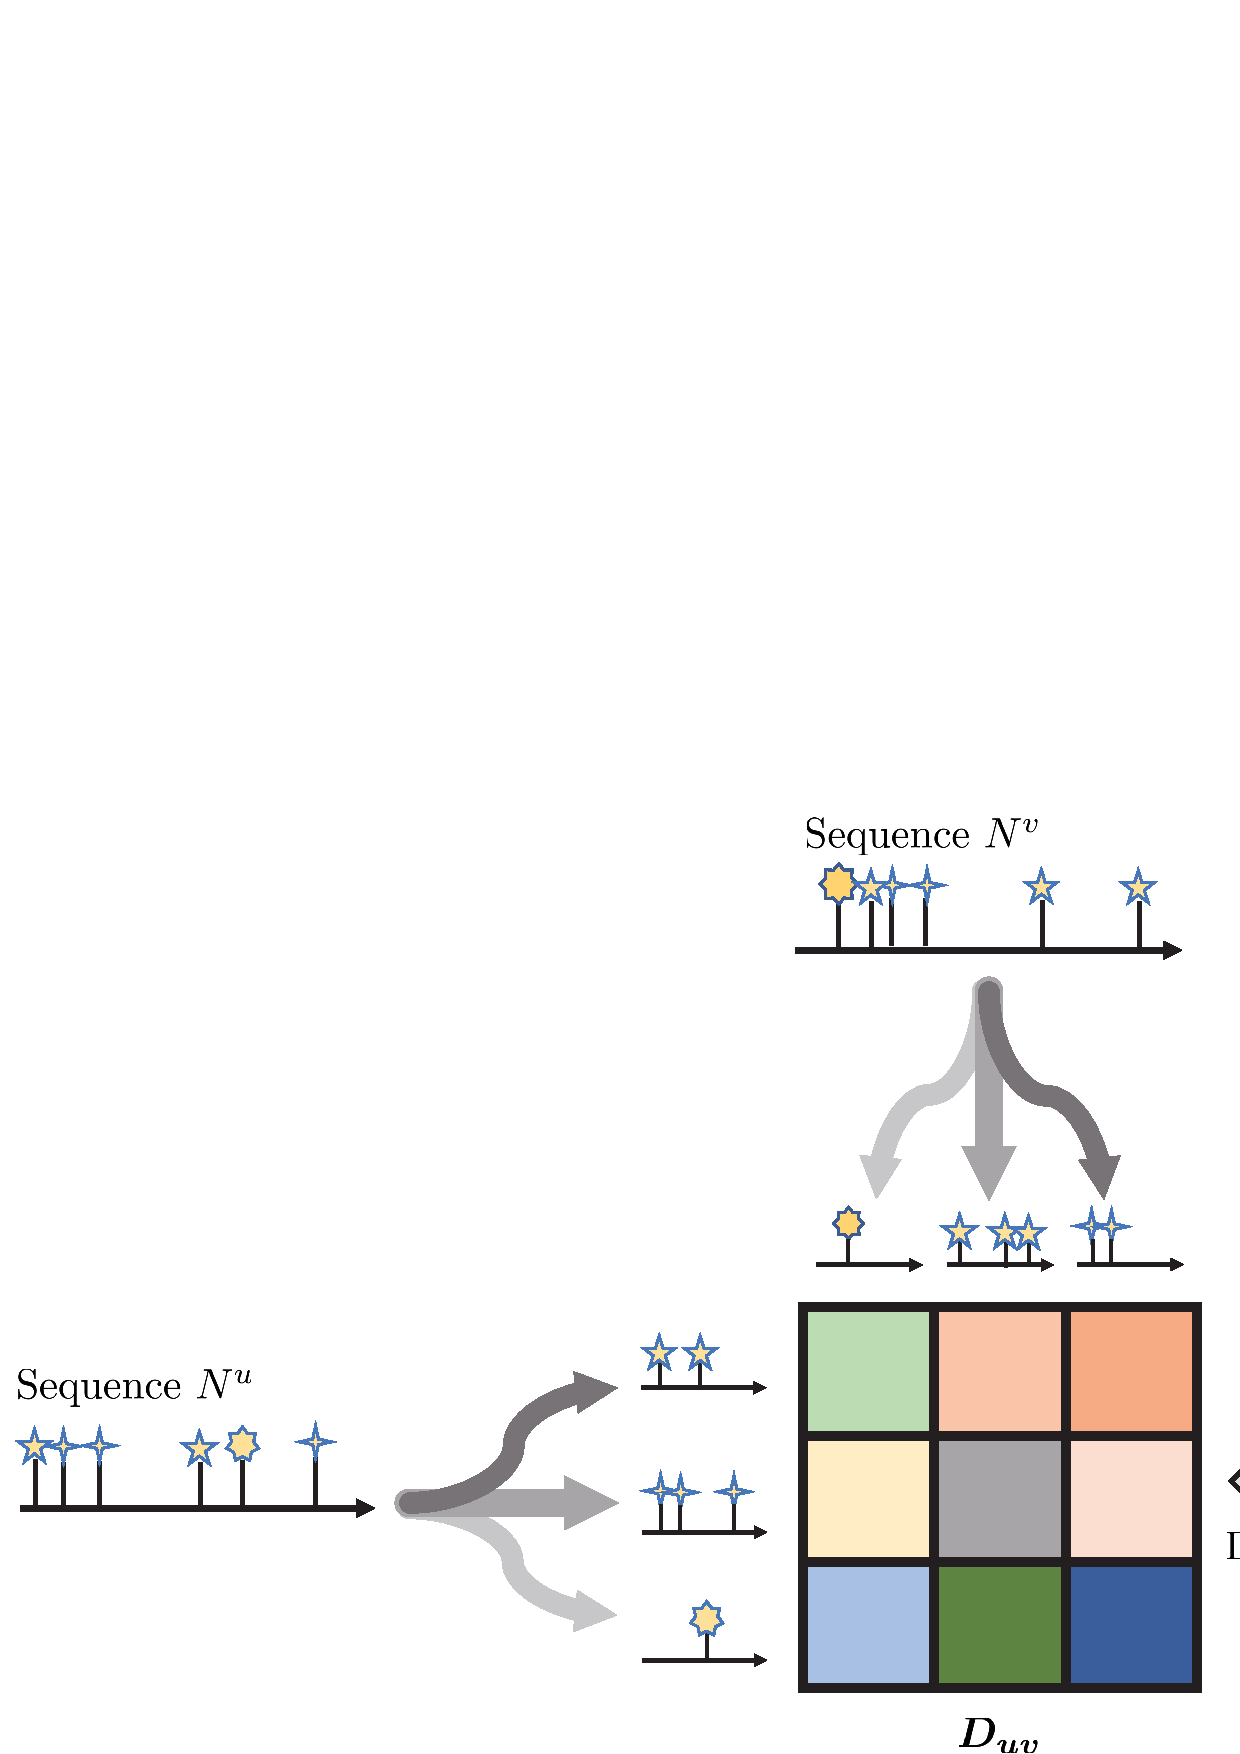
\includegraphics[width=0.9\linewidth]{figure2.jpg}}
\vspace{-10pt}
\caption{The top-k exact match accuracy (\%).}
\label{fig1}
\end{figure}
    
\end{frame}

\end{document}	% Done!

